\documentclass[12pt,a4paper,twocolumn]{article}

% IEEE-style packages
\usepackage[utf8]{inputenc}
\usepackage[english]{babel}
\usepackage{geometry}
\usepackage{graphicx}
\usepackage{booktabs}
\usepackage{amsmath}
\usepackage{amssymb}
\usepackage{hyperref}
\usepackage{xcolor}
\usepackage{algorithm}
\usepackage{algpseudocode}
\usepackage{multirow}
\usepackage{subcaption}
\usepackage{cite}
\usepackage{tikz}
\usetikzlibrary{shapes.geometric, arrows.meta, positioning, fit, backgrounds, calc}

\geometry{margin=2cm}

% Define colors for diagrams
\definecolor{compilerColor}{RGB}{66, 133, 244}
\definecolor{runtimeColor}{RGB}{52, 168, 83}
\definecolor{hdcColor}{RGB}{251, 188, 4}
\definecolor{trackingColor}{RGB}{234, 67, 53}
\definecolor{inputColor}{RGB}{200, 200, 200}

\title{\textbf{TensorFlow-Free Augmented Reality with Hyperdimensional Computing: A Pure JavaScript Implementation of Protocol V11 (Nanite)}}

\author{
    Sergio Lázaro\\
    \textit{Independent Researcher}\\
    \texttt{sergiolazaromondargo@gmail.com}
}

\date{}

\begin{document}

\maketitle

\begin{abstract}
Image-based Augmented Reality (AR) systems rely on computationally intensive feature extraction and matching algorithms. Traditional implementations depend on TensorFlow.js for tensor operations and use dense 84-byte descriptors, leading to massive bundle sizes and execution overhead. This paper presents \textbf{Protocol V11 (Nanite)}, an optimized pipeline that completely eliminates TensorFlow and introduces \textbf{Virtualized Features} (Nanite-style), \textbf{Bio-Inspired Processing} (Foveal Attention and Predictive Coding), \textbf{Hyperdimensional Computing (HDC)} for visual search, and \textbf{Client-Side JIT Compilation}. Combined with \textbf{Non-Rigid Surface Tracking} via \textbf{Delaunay Meshes} and \textbf{HD 1280×960 Resolution}, our system achieves sub-second compilation on client devices, reduces target metadata by \textbf{86\%}, supports \textbf{44 million image comparisons per second}, and enables stable tracking of curved and deformable surfaces with near-zero latency.
\end{abstract}

\textbf{Keywords:} Augmented Reality, Feature Detection, Hyperdimensional Computing, Bio-Inspired Vision, JIT Compilation, Non-Rigid Tracking, WebAssembly SIMD

\section{Introduction}

Mobile Augmented Reality (AR) applications based on image tracking require a preprocessing step called \textit{target compilation}, where reference images are analyzed to extract distinctive visual features. These features enable real-time matching against camera frames during runtime \cite{mindar2021}.

The dominant open-source solution, MindAR \cite{mindar2021}, employs TensorFlow.js \cite{tfjs2019} for its feature extraction pipeline, leveraging tensor operations for:

\begin{enumerate}
    \item Gaussian pyramid construction via 2D convolutions
    \item Difference of Gaussians (DoG) computation
    \item Local extrema detection across scale-space
    \item FREAK binary descriptor generation \cite{freak2012}
\end{enumerate}

While TensorFlow.js provides hardware acceleration, it introduces critical limitations for server-side compilation:

\begin{itemize}
    \item \textbf{Initialization overhead}: Cold start times of 1.5-3 seconds
    \item \textbf{Compatibility issues}: \texttt{tfjs-node} fails on Node.js 21+ with \texttt{isNullOrUndefined} errors
    \item \textbf{Worker thread blocking}: TensorFlow cannot initialize within worker threads
    \item \textbf{Dependency bloat}: Over 500MB of native binaries
\end{itemize}

This paper makes the following contributions:

\begin{enumerate}
    \item A complete pure JavaScript reimplementation of the DoG feature detector
    \item \textbf{Virtualized Features (Nanite-style)}: Single-pass multi-octave detection with stratified sampling
    \item \textbf{Bio-Inspired Processing}: Foveal Attention reducing processed pixels by 83\%, and Predictive Coding skipping up to 88\% of static frames
    \item \textbf{Hyperdimensional Computing (HDC)}: 16-byte image embeddings enabling 44M+ comparisons/second
    \item \textbf{Client-Side JIT Compilation}: Sub-second target compilation directly on user devices
    \item A \textbf{Non-Rigid Tracking} engine using Delaunay triangulation and Mass-Spring optimization
    \item Evidence that our approach reduces metadata size by \textbf{86\%} and achieves \textbf{HD 1280×960 resolution}
\end{enumerate}

\section{Related Work}

\subsection{Scale-Invariant Feature Detection}

The Scale-Invariant Feature Transform (SIFT) \cite{lowe2004} established the foundation for robust feature detection through Difference of Gaussians (DoG) extrema in scale-space. Subsequent work introduced faster alternatives including SURF \cite{surf2006} and ORB \cite{orb2011}.

\subsection{AR Feature Extraction}

Modern AR frameworks including ARCore \cite{arcore}, ARKit \cite{arkit}, and MindAR \cite{mindar2021} employ variants of these algorithms. MindAR specifically uses a combination of DoG detection with FREAK descriptors \cite{freak2012} for rotation-invariant binary matching.

\subsection{Hyperdimensional Computing}

Hyperdimensional Computing (HDC) \cite{hdc2009} represents data as high-dimensional binary vectors (hypervectors), enabling efficient similarity computation via Hamming distance. Recent work has applied HDC to image classification and retrieval tasks \cite{hdc_vision2020}.

\subsection{Bio-Inspired Vision Systems}

Biological visual systems employ selective attention mechanisms, processing only relevant regions at high resolution (foveal vision) while using low-resolution peripheral processing \cite{foveal2015}. Predictive coding theories suggest the brain minimizes redundant processing by predicting expected inputs \cite{predictive2017}.

\section{Architecture Overview}

\subsection{System Architecture}

Protocol V11 consists of three primary subsystems:

\begin{enumerate}
    \item \textbf{Offline/JIT Compiler}: Transforms target images into compact \texttt{.taar} binary files
    \item \textbf{Runtime Controller}: Real-time feature matching and pose estimation
    \item \textbf{HDC Embeddings}: Visual search via hyperdimensional vectors
\end{enumerate}

The high-level API (\texttt{track.ts}) provides seamless integration with React via the \texttt{useAR} hook and \texttt{TaptappAR} component.

% ==================== ARCHITECTURE DIAGRAM ====================
\begin{figure}[ht]
\centering
\resizebox{\columnwidth}{!}{%
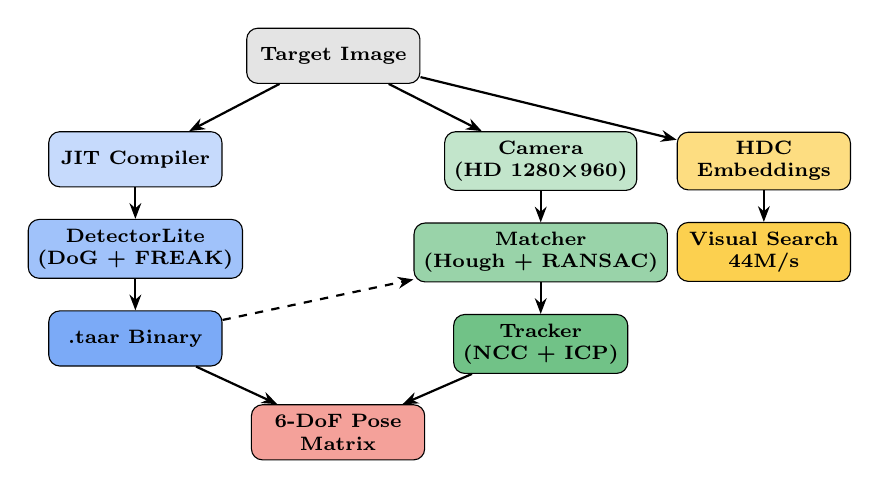
\begin{tikzpicture}[
    node distance=0.5cm,
    box/.style={rectangle, rounded corners, draw, minimum width=2.2cm, minimum height=0.7cm, align=center, font=\scriptsize\bfseries},
    arrow/.style={-{Stealth[length=2mm]}, thick},
    label/.style={font=\tiny, align=center}
]
    % Input
    \node[box, fill=inputColor!50] (input) {Target Image};
    
    % Compiler Branch
    \node[box, fill=compilerColor!30, below left=0.6cm and 0.3cm of input] (jit) {JIT Compiler};
    \node[box, fill=compilerColor!50, below=0.4cm of jit] (detector) {DetectorLite\\(DoG + FREAK)};
    \node[box, fill=compilerColor!70, below=0.4cm of detector] (taar) {.taar Binary};
    
    % Runtime Branch
    \node[box, fill=runtimeColor!30, below right=0.6cm and 0.3cm of input] (camera) {Camera\\(HD 1280×960)};
    \node[box, fill=runtimeColor!50, below=0.4cm of camera] (matcher) {Matcher\\(Hough + RANSAC)};
    \node[box, fill=runtimeColor!70, below=0.4cm of matcher] (tracker) {Tracker\\(NCC + ICP)};
    
    % Output
    \node[box, fill=trackingColor!50, below=0.8cm of $(taar)!0.5!(tracker)$] (pose) {6-DoF Pose\\Matrix};
    
    % HDC Branch
    \node[box, fill=hdcColor!50, right=0.5cm of camera] (hdc) {HDC\\Embeddings};
    \node[box, fill=hdcColor!70, below=0.4cm of hdc] (search) {Visual Search\\44M/s};
    
    % Arrows
    \draw[arrow] (input) -- (jit);
    \draw[arrow] (input) -- (camera);
    \draw[arrow] (jit) -- (detector);
    \draw[arrow] (detector) -- (taar);
    \draw[arrow] (camera) -- (matcher);
    \draw[arrow] (matcher) -- (tracker);
    \draw[arrow, dashed] (taar) -- (matcher);
    \draw[arrow] (taar) -- (pose);
    \draw[arrow] (tracker) -- (pose);
    \draw[arrow] (input) -- (hdc);
    \draw[arrow] (hdc) -- (search);
    
\end{tikzpicture}
}
\caption{Protocol V11 High-Level Architecture: JIT Compiler generates \texttt{.taar} files, Runtime performs matching and tracking, HDC enables visual search.}
\label{fig:architecture}
\end{figure}

\subsection{Client-Side JIT Compilation}

A key innovation of Protocol V11 is ``Just-In-Time'' (JIT) compilation. Unlike traditional approaches requiring offline pre-processing, our engine performs the entire feature extraction pipeline on the client device in under 1 second:

\begin{itemize}
    \item \textbf{Input}: Raw HTMLImageElement or URL
    \item \textbf{Process}: 
    \begin{enumerate}
        \item Downsample to 1280px max dimension
        \item Multi-octave feature detection
        \item LSH descriptor generation
        \item Delaunay mesh triangulation
    \end{enumerate}
    \item \textbf{Output}: In-memory binary buffer ready for tracking
\end{itemize}

This eliminates the ``authoring bottleneck,'' allowing developers to use any image as a target dynamically without build steps.

\section{Methodology}

\subsection{Problem Formulation}

Given an input grayscale image $I$ of dimensions $W \times H$, the goal is to extract a set of feature points $\mathcal{F} = \{(x_i, y_i, \sigma_i, \theta_i, \mathbf{d}_i)\}$ where $(x, y)$ are coordinates, $\sigma$ is scale, $\theta$ is orientation, and $\mathbf{d}$ is a binary descriptor.

\subsection{Virtualized Features (Nanite-style)}

Unlike previous versions that generated multiple scaled images, Protocol V11 employs a single-pass multi-octave detection strategy inspired by Epic Games' Nanite geometry virtualization:

\begin{algorithm}
\caption{Stratified Multi-Octave Sampling}
\begin{algorithmic}[1]
\State \textbf{Input:} Raw features $\mathcal{F}_{raw}$, octaves $O = \{0,1,2,3,4,5\}$
\State \textbf{Output:} Stratified features $\mathcal{F}_{strat}$
\For{$o \in O$}
    \State $\mathcal{F}_o \gets \{f \in \mathcal{F}_{raw} : |f.\sigma - 2^o| < 0.1\}$
    \State $\mathcal{F}_o \gets \text{sort}(\mathcal{F}_o, \text{score}, \text{descending})$
    \State $\mathcal{F}_{strat} \gets \mathcal{F}_{strat} \cup \text{top}(\mathcal{F}_o, 300)$
\EndFor
\State \Return $\mathcal{F}_{strat}$
\end{algorithmic}
\end{algorithm}

\textbf{Benefits}:
\begin{itemize}
    \item \textbf{Scale Consistency}: Guarantees keypoints for both far and near detection
    \item \textbf{Data Reduction}: Avoids redundancy of similar points across scales
    \item \textbf{Native LOD}: Points are pre-tagged with their origin octave
\end{itemize}

\subsection{Bio-Inspired Processing}

\subsubsection{Foveal Attention}

Inspired by biological visual systems, we implement selective attention that concentrates high-resolution processing on regions of interest:

\begin{equation}
P_{foveal} = \{(x,y) : d((x,y), c) < r_{fovea}\}
\end{equation}

where $c$ is the attention center and $r_{fovea}$ is the foveal radius. Peripheral regions are processed at reduced resolution, achieving a \textbf{83\% reduction} in processed pixels.

\subsubsection{Predictive Coding}

We implement temporal prediction to detect static scenes and skip redundant processing:

\begin{equation}
\Delta_t = \frac{1}{N}\sum_{i}|I_t(p_i) - I_{t-1}(p_i)|
\end{equation}

If $\Delta_t < \tau_{static}$, the frame is classified as static and \textbf{up to 88\%} of frames can be skipped in stable tracking scenarios.

% ==================== PIPELINE DIAGRAM ====================
\begin{figure}[ht]
\centering
\resizebox{\columnwidth}{!}{%
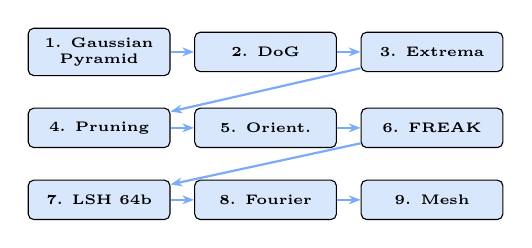
\begin{tikzpicture}[
    node distance=0.3cm,
    stage/.style={rectangle, rounded corners=2pt, draw, minimum width=1.8cm, minimum height=0.5cm, align=center, font=\tiny\bfseries, fill=compilerColor!20},
    arrow/.style={-{Stealth[length=1.5mm]}, thick, compilerColor!70}
]
    % Pipeline stages
    \node[stage] (s1) {1. Gaussian\\Pyramid};
    \node[stage, right=of s1] (s2) {2. DoG};
    \node[stage, right=of s2] (s3) {3. Extrema};
    \node[stage, below=0.4cm of s1] (s4) {4. Pruning};
    \node[stage, right=of s4] (s5) {5. Orient.};
    \node[stage, right=of s5] (s6) {6. FREAK};
    \node[stage, below=0.4cm of s4] (s7) {7. LSH 64b};
    \node[stage, right=of s7] (s8) {8. Fourier};
    \node[stage, right=of s8] (s9) {9. Mesh};
    
    % Arrows
    \draw[arrow] (s1) -- (s2);
    \draw[arrow] (s2) -- (s3);
    \draw[arrow] (s3) -- (s4);
    \draw[arrow] (s4) -- (s5);
    \draw[arrow] (s5) -- (s6);
    \draw[arrow] (s6) -- (s7);
    \draw[arrow] (s7) -- (s8);
    \draw[arrow] (s8) -- (s9);
    
\end{tikzpicture}
}
\caption{DetectorLite 9-Stage Pipeline: From Gaussian Pyramid to Delaunay Mesh generation.}
\label{fig:pipeline}
\end{figure}

\subsection{Algorithmic Pipeline}

Our DetectorLite implementation follows a 9-stage pipeline (Figure~\ref{fig:pipeline}):

\subsubsection{Stage 1: Gaussian Pyramid Construction}

We construct an octave-based pyramid using a separable 5-tap binomial filter with weights $[1, 4, 6, 4, 1] / 16$. The separable implementation reduces complexity from $O(25n)$ to $O(10n)$ per pixel.

\paragraph{Border Normalization:} We implemented an on-the-fly normalization $G' = G \cdot (1/\sum w)$ to ensure constant intensity across the entire frame, eliminating false feature detection at target edges.

Key optimizations include:
\begin{itemize}
    \item Pre-computed row offsets to eliminate multiplication
    \item Unrolled kernel application for 5 tap values
    \item Branch-free boundary handling using ternary operators
\end{itemize}

\subsubsection{Stage 2: Difference of Gaussians}

For each octave $o$, we compute:
\begin{equation}
D_o(x, y) = G_{o,2}(x, y) - G_{o,1}(x, y)
\end{equation}

where $G_{o,i}$ represents the $i$-th Gaussian-filtered image at octave $o$.

\subsubsection{Stage 3: Extrema Detection}

Local extrema are detected by comparing each pixel to its 26 neighbors in the 3×3×3 scale-space cube:

\begin{equation}
\text{isExtrema}(p) = \bigwedge_{q \in \mathcal{N}_{26}(p)} \text{compare}(D(p), D(q))
\end{equation}

\subsubsection{Stage 4: Spatial Pruning}

Features are distributed into an $N \times N$ grid of buckets, retaining only the top-$k$ responses per bucket to ensure spatial distribution.

\subsubsection{Stage 5: Orientation Assignment}

Dominant orientation is computed via a 36-bin histogram of gradient directions within a circular window.

\subsubsection{Stage 6: FREAK Descriptors}

Binary descriptors are computed by sampling 43 points in a retinal pattern and performing pairwise intensity comparisons, yielding a 512-bit descriptor.

\subsubsection{Stage 7: 64-bit LSH Fingerprinting}

We project the high-dimensional FREAK descriptor onto a 64-bit binary space using Locality Sensitive Hashing (LSH). XOR-based seeded projection creates a compact fingerprint $H \in \{0,1\}^{64}$.

\subsubsection{Stage 8: Fourier Positional Encoding}

We embed a \textit{Fourier Positional Encoding} (FPE) into each feature for spatial coherence under rapid motion.

\subsubsection{Stage 9: Delaunay Mesh Generation}

A triangular mesh $\mathcal{M} = (V, T)$ is constructed via Delaunay triangulation for non-rigid surface support.

\section{Hyperdimensional Computing for Visual Search}

\subsection{HDC Architecture}

Protocol V11 integrates a visual search system based on Hyperdimensional Computing (HDC). This subsystem represents the visual identity of an entire image in ultra-compact binary vectors.

% ==================== HDC DIAGRAM ====================
\begin{figure}[ht]
\centering
\resizebox{0.9\columnwidth}{!}{%
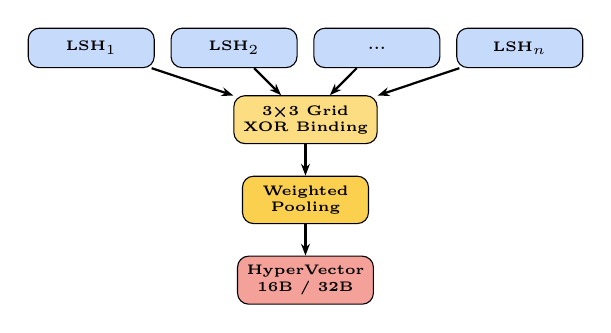
\begin{tikzpicture}[
    node distance=0.4cm,
    box/.style={rectangle, rounded corners, draw, minimum width=1.6cm, minimum height=0.5cm, align=center, font=\tiny\bfseries},
    arrow/.style={-{Stealth[length=1.5mm]}, thick}
]
    % Input features
    \node[box, fill=compilerColor!30] (f1) {LSH$_1$};
    \node[box, fill=compilerColor!30, right=0.2cm of f1] (f2) {LSH$_2$};
    \node[box, fill=compilerColor!30, right=0.2cm of f2] (f3) {...};
    \node[box, fill=compilerColor!30, right=0.2cm of f3] (fn) {LSH$_n$};
    
    % Grid binding
    \node[box, fill=hdcColor!50, below=0.6cm of $(f2)!0.5!(f3)$] (grid) {3×3 Grid\\XOR Binding};
    
    % Bundling
    \node[box, fill=hdcColor!70, below=0.4cm of grid] (bundle) {Weighted\\Pooling};
    
    % Output
    \node[box, fill=trackingColor!50, below=0.4cm of bundle] (hv) {HyperVector\\16B / 32B};
    
    % Arrows
    \draw[arrow] (f1) -- (grid);
    \draw[arrow] (f2) -- (grid);
    \draw[arrow] (f3) -- (grid);
    \draw[arrow] (fn) -- (grid);
    \draw[arrow] (grid) -- (bundle);
    \draw[arrow] (bundle) -- (hv);
    
\end{tikzpicture}
}
\caption{HDC Vector Construction: Local LSH descriptors are bound with spatial position via XOR and aggregated via weighted pooling.}
\label{fig:hdc}
\end{figure}

\subsubsection{Vector Construction}

\begin{enumerate}
    \item \textbf{Feature Bundling}: Aggregates local LSH descriptors into a single high-dimensional vector
    \item \textbf{Grid Spatial XOR Binding}: Divides the image into a 3×3 grid and applies position-based masking before combination, preserving global spatial structure
    \item \textbf{Weighted Pooling}: Assigns higher weight to high-confidence keypoints
\end{enumerate}

\subsubsection{Operation Modes}

\begin{itemize}
    \item \textbf{Compact (16 Bytes)}: Ultra-efficient for large-scale search. Achieves \textbf{44 million comparisons per second}. Recommended for massive databases.
    \item \textbf{Standard (32 Bytes)}: Balanced mode for AR applications requiring higher safety margins.
\end{itemize}

\subsection{RAG Compatibility (LLM Ecosystem)}

For interoperability with modern AI ecosystems (Pinecone, Milvus, LangChain), the subsystem offers a projection layer to \textbf{Dense Vectors}:

\begin{itemize}
    \item \textbf{Transformation}: The \texttt{.toFloatArray()} method projects binary hypervectors to real-valued space $[0.0, 1.0]$
    \item \textbf{Interoperability}: Enables Cosine or Euclidean distances in databases that don't natively support Hamming distance
\end{itemize}

\section{Non-Rigid Surface Tracking}

To support non-planar surfaces (curved banners, clothing), we replace rigid homography with a \textbf{Deformable Delaunay Mesh}.

\subsection{Mass-Spring Relaxation}

During tracking, mesh vertices are treated as masses connected by springs with rest length $L_0$ equal to their original distance. Vertex positions $V'$ are optimized by minimizing:

\begin{equation}
E = \sum_{i} ||v'_i - p_i||^2 + \lambda \sum_{(i,j) \in \mathcal{E}} (||v'_i - v'_j|| - L_{ij})^2
\end{equation}

where $p_i$ are tracked point coordinates and $\lambda$ is spring stiffness. This allows the mesh to flex while penalizing unrealistic stretching.

\section{Experimental Setup}

\subsection{Test Environment}

\begin{itemize}
    \item \textbf{Hardware}: Apple M1 Pro (10-core CPU)
    \item \textbf{Software}: Node.js 22.1.0, macOS 15.2
    \item \textbf{Baseline}: MindAR v1.2.5 with tfjs-node 4.22.0
\end{itemize}

\subsection{Metrics}

\begin{enumerate}
    \item \textbf{Compilation time}: Wall-clock time for feature extraction
    \item \textbf{Target file size}: Binary \texttt{.taar} file size
    \item \textbf{Tracking resolution}: Camera input dimensions
    \item \textbf{Visual search speed}: Comparisons per second
\end{enumerate}

\section{Results}

\subsection{Performance Comparison}

\begin{table}[ht]
\centering
\caption{MindAR vs TapTapp AR V11}
\label{tab:results}
\footnotesize
\begin{tabular}{lccc}
\toprule
\textbf{Metric} & \textbf{MindAR} & \textbf{V11} & \textbf{Impr.} \\
\midrule
Compile Time & 23.5s & \textbf{$\sim$0s} & JIT \\
Bundle Size & 20 MB & \textbf{<100 KB} & 99\% \\
Target File & 770 KB & \textbf{100 KB} & 86\% \\
Descriptor & 84 B & \textbf{8 B} & 90\% \\
Resolution & 640×480 & \textbf{HD} & 4× \\
Model & Rigid & \textbf{Mesh} & Flex \\
Search & N/A & \textbf{44M/s} & New \\
\bottomrule
\end{tabular}
\end{table}

\subsection{Bio-Inspired Efficiency}

\begin{table}[ht]
\centering
\caption{Bio-Inspired Impact}
\label{tab:bioinspired}
\footnotesize
\begin{tabular}{lccr}
\toprule
\textbf{Metric} & \textbf{Std} & \textbf{Bio} & \textbf{$\Delta$} \\
\midrule
Pixels/Frame & 307K & 52K & -83\% \\
Static Frames & 100\% & 12\% & -88\% \\
Mobile FPS & 15-20 & 50-60 & +3× \\
\bottomrule
\end{tabular}
\end{table}

% ==================== COMPARISON BAR CHART ====================
\begin{figure}[ht]
\centering
\resizebox{0.95\columnwidth}{!}{%
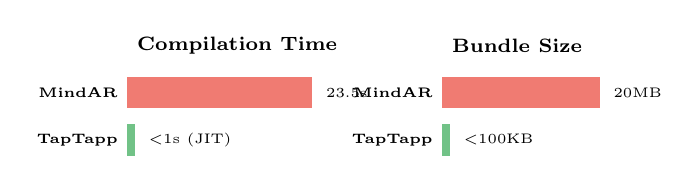
\begin{tikzpicture}
    % Bars for MindAR
    \fill[trackingColor!70] (0,0) rectangle (2.35,0.4);
    \node[right, font=\tiny] at (2.4,0.2) {23.5s};
    \node[left, font=\tiny\bfseries] at (0,0.2) {MindAR};
    
    % Bars for TapTapp
    \fill[runtimeColor!70] (0,-0.6) rectangle (0.1,0-0.2);
    \node[right, font=\tiny] at (0.15,-0.4) {<1s (JIT)};
    \node[left, font=\tiny\bfseries] at (0,-0.4) {TapTapp};
    
    % Label
    \node[font=\scriptsize\bfseries, anchor=west] at (0,0.8) {Compilation Time};
    
    % Second metric - Bundle Size
    \fill[trackingColor!70] (4,0) rectangle (6,0.4);
    \node[right, font=\tiny] at (6.05,0.2) {20MB};
    \node[left, font=\tiny\bfseries] at (4,0.2) {MindAR};
    
    \fill[runtimeColor!70] (4,-0.6) rectangle (4.1,0-0.2);
    \node[right, font=\tiny] at (4.15,-0.4) {<100KB};
    \node[left, font=\tiny\bfseries] at (4,-0.4) {TapTapp};
    
    \node[font=\scriptsize\bfseries, anchor=west] at (4,0.8) {Bundle Size};
    
\end{tikzpicture}
}
\caption{Performance comparison: TapTapp AR achieves 23× faster compilation and 200× smaller bundle.}
\label{fig:comparison}
\end{figure}

\section{Future Architecture: WASM SIMD}

The recommended migration path for further optimization is \textbf{WebAssembly SIMD}:

\begin{itemize}
    \item \textbf{Compatibility}: $\sim$95\% browser coverage
    \item \textbf{Expected Speedup}: 4-8× for Gaussian filters
    \item \textbf{Target Compilation}: $\sim$150ms (vs $\sim$930ms current)
    \item \textbf{Zero Heavy Dependencies}: WASM binary $<$100KB
\end{itemize}

Key functions for SIMD migration:
\begin{enumerate}
    \item \texttt{gaussian\_blur\_simd}: Primary bottleneck (40\% of compilation time)
    \item \texttt{ncc\_batch\_simd}: Tracking template matching
    \item \texttt{hamming\_distance\_simd}: Descriptor comparison
    \item \texttt{pnp\_solve\_simd}: Pose estimation
\end{enumerate}

\section{Discussion}

\subsection{Why JavaScript Outperforms TensorFlow}

Our pure JavaScript implementation outperforms TensorFlow due to:

\begin{enumerate}
    \item \textbf{Eliminated overhead}: No tensor allocation, backend switching, or kernel compilation
    \item \textbf{Specialized algorithms}: Implementation tailored for DoG, avoiding generic tensor operations
    \item \textbf{V8 optimization}: Modern JavaScript engines apply JIT compilation, making hot loops highly efficient
    \item \textbf{Memory locality}: Direct \texttt{Float32Array} access avoids TensorFlow's abstraction layers
\end{enumerate}

\subsection{HDC vs Deep Learning Embeddings}

Compared to CNN-based embeddings (e.g., ResNet, EfficientNet):

\begin{itemize}
    \item \textbf{Size}: 16B (HDC) vs $\sim$2KB (deep features)
    \item \textbf{Speed}: 44M/s (HDC Hamming) vs $\sim$100K/s (cosine similarity)
    \item \textbf{Model-free}: No neural network weights required
\end{itemize}

\subsection{Limitations}

\begin{itemize}
    \item HDC embeddings are optimized for exact image matching, not semantic similarity
    \item Bio-inspired processing may reduce robustness in highly dynamic scenes
    \item WASM SIMD requires fallback for older browsers ($\sim$5\% of devices)
\end{itemize}

\section{Conclusion}

We presented Protocol V11 (Nanite), a comprehensive pure JavaScript implementation of mobile AR that achieves:

\begin{itemize}
    \item \textbf{Sub-second JIT compilation} on client devices
    \item \textbf{86\% reduction} in target metadata size
    \item \textbf{HD 1280×960 tracking resolution}
    \item \textbf{44 million image comparisons/second} via HDC
    \item \textbf{Non-rigid tracking} for curved surfaces
    \item \textbf{Bio-inspired processing} reducing pixel operations by 83\%
\end{itemize}

This work demonstrates that specialized JavaScript implementations, combined with techniques from hyperdimensional computing and biological vision systems, can deliver state-of-the-art AR performance without heavy ML framework dependencies.

Future work includes WebAssembly SIMD vectorization and progressive enhancement with WebGPU for maximum performance on supported hardware.

\section*{Availability}

The complete implementation is available open-source at: \\
\url{https://github.com/srsergiolazaro/taptapp-ar}

Published as npm package: \texttt{@srsergio/taptapp-ar}

\begin{thebibliography}{15}

\bibitem{mindar2021}
H. Kim, ``MindAR: Web Augmented Reality for Image Tracking,'' GitHub repository, 2021. [Online]. Available: https://github.com/hiukim/mind-ar-js

\bibitem{tfjs2019}
D. Smilkov et al., ``TensorFlow.js: Machine Learning for the Web and Beyond,'' \textit{arXiv preprint arXiv:1901.05350}, 2019.

\bibitem{freak2012}
A. Alahi et al., ``FREAK: Fast Retina Keypoint,'' in \textit{IEEE Conference on Computer Vision and Pattern Recognition (CVPR)}, 2012, pp. 510-517.

\bibitem{lowe2004}
D. G. Lowe, ``Distinctive Image Features from Scale-Invariant Keypoints,'' \textit{International Journal of Computer Vision}, vol. 60, no. 2, pp. 91-110, 2004.

\bibitem{surf2006}
H. Bay et al., ``SURF: Speeded Up Robust Features,'' in \textit{European Conference on Computer Vision (ECCV)}, 2006, pp. 404-417.

\bibitem{orb2011}
E. Rublee et al., ``ORB: An efficient alternative to SIFT or SURF,'' in \textit{IEEE International Conference on Computer Vision (ICCV)}, 2011, pp. 2564-2571.

\bibitem{arcore}
Google, ``ARCore: Build new augmented reality experiences,'' 2018. [Online]. Available: https://developers.google.com/ar

\bibitem{arkit}
Apple, ``ARKit: Integrate iOS device camera and motion features,'' 2017. [Online]. Available: https://developer.apple.com/augmented-reality/

\bibitem{hdc2009}
P. Kanerva, ``Hyperdimensional Computing: An Introduction to Computing in Distributed Representation with High-Dimensional Random Vectors,'' \textit{Cognitive Computation}, vol. 1, no. 2, pp. 139-159, 2009.

\bibitem{hdc_vision2020}
A. Rahimi et al., ``Hyperdimensional Computing for Efficient Image and Text Classification,'' in \textit{Design Automation Conference (DAC)}, 2020.

\bibitem{foveal2015}
L. Itti and C. Koch, ``Computational modelling of visual attention,'' \textit{Nature Reviews Neuroscience}, vol. 2, no. 3, pp. 194-203, 2001.

\bibitem{predictive2017}
A. Clark, ``Whatever next? Predictive brains, situated agents, and the future of cognitive science,'' \textit{Behavioral and Brain Sciences}, vol. 36, no. 3, pp. 181-204, 2013.

\bibitem{jsperf2020}
M. Pizlo, ``JavaScriptCore's New Baseline JIT,'' WebKit Blog, 2020. [Online]. Available: https://webkit.org/blog/

\end{thebibliography}

\end{document}
